\begin{frame}
  \frametitle{Prior on Composition ($\theta$)}
  \begin{center}
    We need some prior probability distribution on $\theta$.
    \vspace{0.3in}

    A Dirichlet distribution is a common choice for this kind of application.
    However, the Dirichlet distribution doesn't have enough degrees of freedom to represent co-occurrences.
  \end{center}
\end{frame}

\begin{frame}
  \frametitle{Logistic Normal Prior on Composition ($\theta$)}
  \begin{center}
    \begin{equation*}
      \theta = ( \theta_1, \theta_2, \dots \theta_T )
    \end{equation*}

    \begin{equation*}
      \eta \sim \mathcal{N}(\mu, \Sigma)
    \end{equation*}

    $\sigma(\eta)$ transforms the normally distributed $\eta \in \mathbb{R}^T$ \\
    to $\theta \in \mathbb{R}_+^T$ such that $\norm{1}{\theta} = 1$.

    \begin{equation*}
      \theta_i = \sigma(\eta_i) = \frac{e^{\eta_i}}{\sum_{k=1}^{T}e^{\eta_k}}
    \end{equation*}
  \end{center}
\end{frame}

\begin{frame}
  \frametitle{Logistic Normal Prior on Composition ($\theta$)}
  \begin{center}
    Histogram of $\theta_i$
    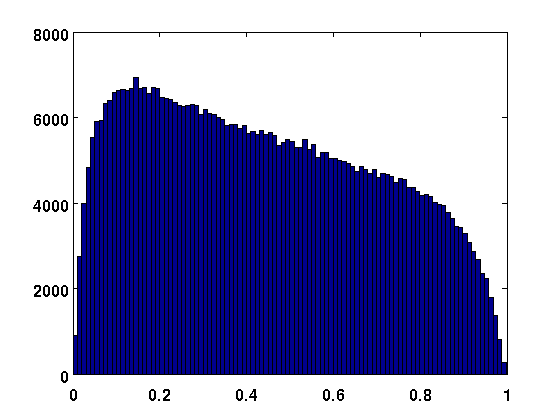
\includegraphics[scale=0.6]{img/log-normal-figs/hist-1.png}
  \end{center}
\end{frame}

\begin{frame}
  \frametitle{Logistic Normal Prior on Composition ($\theta$)}
  \begin{center}
    \vspace{-0.4in}
    \begin{equation*}
      \eta \sim \mathcal{N}(\mu, \Sigma)
    \end{equation*}
    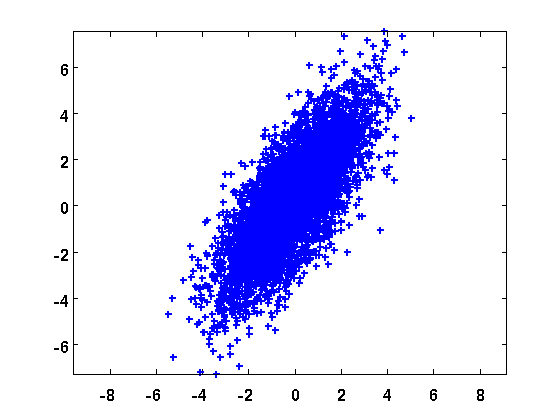
\includegraphics[scale=0.6]{img/log-normal-figs/normal-1.png}
  \end{center}
\end{frame}

\begin{frame}
  \frametitle{Logistic Normal Prior on Composition ($\theta$)}
  \begin{center}
    Histogram of $\theta_i$
    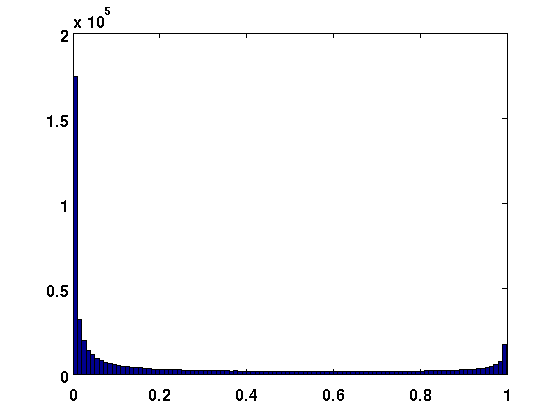
\includegraphics[scale=0.6]{img/log-normal-figs/hist-2.png}
  \end{center}
\end{frame}

\begin{frame}
  \frametitle{Logistic Normal Prior on Composition ($\theta$)}
  \begin{center}
    \vspace{-0.4in}
    \begin{equation*}
      \eta \sim \mathcal{N}(\mu, \Sigma)
    \end{equation*}
    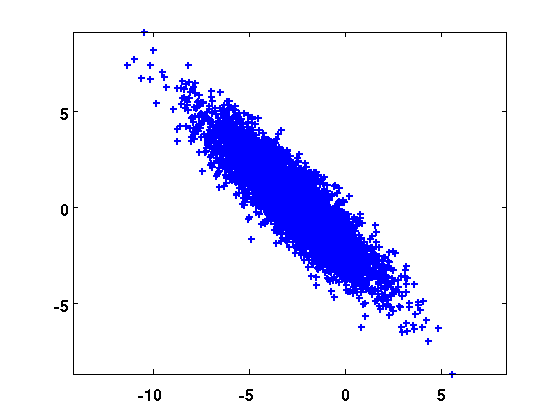
\includegraphics[scale=0.6]{img/log-normal-figs/normal-2.png}
  \end{center}
\end{frame}

%\begin{frame}
%  \frametitle{Inverse of Logistic Transformation}
%  \begin{center}
%    \begin{equation*}
%      \eta \sim \mathcal{N}(\mu, \Sigma)
%    \end{equation*}
%
%    \begin{equation*}
%      \theta_i = \sigma(\eta_i) = \frac{e^{\eta_i}}{\sum_{k=1}^{T}e^{\eta_k}}
%    \end{equation*}
%
%    \begin{equation*}
%      \eta_i = \sigma^{-1}(\theta_i)
%    \end{equation*}
%
%    \begin{equation*}
%      \eta_i \propto \ln \theta_i
%    \end{equation*}
%
%    WTF! THIS DOESN'T SEEM TO WORK! \\
%    HELP ME PROFESSOR WILLIAMS! YOU'RE MY ONLY HOPE!
%  \end{center}
%\end{frame}
